

%!TEX root = ../dissertation.tex
\chapter{FUNCTIONAL DATA ANALYSIS APPROACH TO LAND COVER CLASSIFICATION IN INDIA USING MERIS TERRESTRIAL CHLOROPHYLL INDEX} \label{phenology}

\section{Introduction}

Phenology is the study of annual life-cycles of terrestrial vegetation and how they are effected by climate change or other environmental variables. Understanding vegetation phenology and its spatio-temporal variation is required to reveal and predict ongoing changes in Earth system dynamics (\cite{Jeganathan:2010gqa}). While ground based phenological measurements can provide information on specific species with high temporal resolution it is challenging to get rich spatial information (\cite{Studer:2007hd}). Monitoring phenology at the ground level also suffers from subjectivity, and a difficulty to relate field data with climatic variables (\cite{Jeganathan:2010gqa}). Remotely sensed data, on the other hand, can provide spatial information at local and global scales, but satellite based equipment typically has a lower limit to the spatial resolution it can achieve, thus making it challenging to associate a spatial unit with a species or vegetation type. 

Observed phenological patterns are known to be closely connected to the type of vegetation (\cite{Dash:2010kva}), thus land cover classification plays an important role in understanding species-specific effects due to climate change. For example, \cite{Dash:2010kva} pointed out an inconsitent effect on onset of greeness in the lower latitudes over India and noted that it could possibly be attributed to misclassification in the landcover map. In order to incorproate land cover information many studies make use of the global land cover database (GLC2000) created in a hugely collabortive effort at the end of the last millenium. The goal of createing the GLC2000 map was to create a freely available high spatial resolution global land cover map that could be used for both scientific research as well as policy development (\cite{Bartholome:2005cq}). 

The construction of the GLC2000 map made use of various classification methods (\cite{Dash:2010kva}), but to our knowledge satellite based phenological measurements have not been used to classify land cover. We describe a method for land cover classification using satellite based phenological measurements by treating the annual time-series data as noisy observations of smooth curves. 

Classification of vegetation type is further complicated due to anthropogenic actions such as deforestation for the purpose of expanding agricultural land, which alters its role in the functioning of the climate system (\cite{Shukla:1990wr}), and drastically changes observed phenological patters due to changes in the type of vegetation as well as cropping cycles. 

\section{Data} 

% (fold)
\label{sec:data} We use Medium Resolution Imaging Spectrometer (MERIS) Terrestrial Chlorophyll Index (MTCI). The data is comprised of 8-day composites at a spatial resolution of 4.6~km for the years 2003-2007 which can be obtained from the NERC Earth Observation Data Centre (NEODC) website (http://www.neodc.rl.ac.uk). The study region we consider is a 230~km~$\times$~230~km subregion of southern India. Land cover type is derived from the Global Landcover 2000 database by [add info on derivation of landcover from 1km GLC200 to 4.6km cells].  Most studies using satellite sensor extracted phenoloical variables used the normalized difference vegetation idex (NDVI) to estimate phenological variables (\cite{Jeyaseelan:2007dh,Saikia:2009cm}). One significant challenge that has been noted using NDVI data is variation in smooth grouth curves due to temporal variation in the presense of cloud, water, snow or shadow (\cite{Goward:1985hr,Huete:2002gy}). An operational European Space Agency Envisat product, the Medium Resolution Imaging Spectrometer (MERIS) Terrestrial Chlorophyll Index (MTCI), has limited sensitivity to atmospheric effects and also soil background and view angle (\cite{Dash:2010kva}). 

\subsection{Data cleaning and processing} % (fold)
\label{sub:data_cleaning_and_processing}

The MTCI data we work with has been preprocessed to deal with erroneous values. The methods used to clean the raw data are described in (\cite{Dash:2010kva}). Valid MTCI data range from about 1 to 6, but due to reasons ranging from local climate fluctuations to sensor malfunction some values were removed from the data and replacement values were included in the data using the mean of the two nearest temporal neighbors. Interpolating values in this manner is not necessary for the methodology we use, because there is neither an assumption of equally spaced time points nor consistent time observations across curves.

% subsection data_cleaning_and_processing (end)
\begin{figure}
	[htbp] \centering 
	\includegraphics[width=0.49\linewidth]{Images-phenology-fda/Satellite/India-current.png} 
	\includegraphics[width=0.49\linewidth]{Images-phenology-fda/Satellite/India-5-12-2000.png} \caption{Satellite image of study region in souther India from 2014 (left) and 2000 (right).} \label{fig:phenology diagram} 
\end{figure}
\begin{figure}
	[htbp] \centering 
	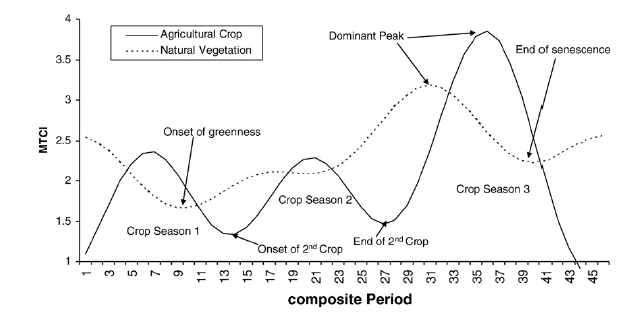
\includegraphics[width=\linewidth]{Images-phenology-fda/PhenoVars_Jegan.png} \caption{Diagram illustrating typical phenology patterns for agricultural land and natural vegetation from \cite{Dash:2010kva}. } \label{fig:phenology diagram} 
\end{figure}
\begin{figure}
	[htbp] \centering 
	\includegraphics[width=\linewidth]{Images-phenology-fda/land_cover.pdf} \caption{Land cover classification at 4.6~km spatial resolution derived from GLC2000 land cover database} \label{fig:land cover} 
\end{figure}
\begin{figure}
	[htbp] \centering 
	\includegraphics[width=\linewidth]{Images-phenology-fda/land_cover_ag_vs_veg.pdf} \caption{Land cover map of the study region aggregated into ``Agriculture'', ``Vegetation'', and ``other''. Grid cells were labeled ``Vegetation'' if their original land cover was Tropical Evergreen, Subtropical Evergreen, Tropical Semievergreen, Tropical Moist Deciduous, or Coastal vegetation. Grid cells were labeled ``Agriculture'' is their original land cover was Rainfed Agriculture, Slope Agriculture, Irrigated Agriculture, or Irrigated Intensive Agriculture. } \label{fig:land cover ag vs. veg} 
\end{figure}
\begin{figure}
	[htbp] \centering 
	\includegraphics[width=\linewidth]{Images-phenology-fda/proportion_agriculture.pdf} \caption{Map of the study region showing the proportion of agricultural land within each of the 4.6~km$\times$4.6~km grid cells based on the GLC2000 land cover database. } \label{fig:proportion agriculture} 
\end{figure}

% section data (end)
\section{Methodology} 

% (fold)
\label{sec:methodology}

In the following we assume $\T$ to be the interval $[0,1]$. Let $X(\cdot)$ be a second order stochastic process with covariance function
\[ C_{0}(s,t)=E([X(s)-E(X(s))][X(t)-E(X(t))]),\mbox{ }\forall s,t\in \T. \]
Further, we assume $X(\cdot)$ is smooth in that it takes values in a reproducing kernel Hilbert space $\H$ with corresponding reproducing kernel $R(s,t)$. 

Let $\{X_{1},X_{2},\dots,X_{N}\}$ be a collection of independent realizations of $X$, and we consider the following observation model with noise
\[ Y_{ij}=X_{i}(t_{ij})+\epsilon_{ij},\mbox{ }j=1,\dots,m;\mbox{ }i=1,\dots,N, \]
where the sampling times correspond to the 8-day composite time points and $\epsilon_{ij}$ are independently and identically distributed measurement errors with mean zero and finite variance $\sigma_{0}^{2}.$ It is further assumed that the random functions $X,$ and measurement errors $\epsilon$ are mutually independent. 

\subsection{Smoothing} 

% (fold)
\label{sub:smoothing}

\subsection{Selecting an appropriate weight} 

% (fold)
\label{sub:selecting_an_appropriate_weight} Define location intensity as the number of locations per unit area (a familiar concept in spatial point processes). In order to quantify the sentiment in the previous paragraph we propose estimating the intensity for each location, denoted by $\gamma_k$, and define a weight function 
\begin{equation}
	w_k = \left(\frac{1}{\gamma_k}\right)^p. 
\end{equation}

Let $\mathbf{W} = diag(\mathbf{w}_1, \dots, \mathbf{w}_n)$, then the covariance estimator is adjusted by defining the loss function as 
\begin{equation}
	l_{n}(C)= (\mathbf{b} - \mathbf{C})^T\mathbf{W}(\mathbf{b} - \mathbf{C}). \label{eq:diag weighted loss function} 
\end{equation}
We investigate the effect of adjusting for spatial dependence in this manner by simulating curves from a grid consisting of group of locations that are spars (low point intensity) and a clustered group of locations (high point intensity) shown in Figure~\ref{fig:grid3}. Different levels of spatial dependence are modeled through the value of the range parameter on a exponential covariance function, 
\begin{equation}
	cov(s_j, s_k) = \sigma^2e^{-\frac{\norm{s_j - s_k}}{r}}. 
\end{equation}

Figure~\ref{fig:exp_corr_funs} shows the exponential correlation functions that correspond to the range values used ($r = 0.1, 0.2, 0.3$; $\sigma^2=1$). We used 20 observations per curve and a negligible noise variance. 

% plot of exponential covariance functions
\begin{figure}
	\begin{center}
		\includegraphics[width= 
		\textwidth]{Images-ordinary-kriging/Plots/exp_corr_funs.pdf} 
	\end{center}
	\caption{Exponential covariance functions used in the simulation.} \label{fig:exp_corr_funs} 
\end{figure}

% plots of MSE vs spatial weight values for different values of spatial dependence
\begin{figure}
	\begin{center}
		\includegraphics[width= 
		\textwidth]{Images-ordinary-kriging/Plots/MSE_trends.pdf} 
	\end{center}
	\caption{The x-axis shows the value of the scale parameter, $p$, in the weight function. Large values of $p$ correspond to smaller weights for curves in high point intensity areas. The y-axis shows the average integrated square error for the covariance estimator. The error bars show +/- two standard errors.} \label{fig:MSE_trends} 
\end{figure}

% subsection selecting_an_appropriate_weight (end)
% subsection smoothing (end)
\subsection{Land Cover Classification} 

% (fold)
\label{sub:land_cover_classification}
\begin{figure}
	[htbp] \centering 
	\includegraphics[width=\linewidth]{Images-phenology-fda/india_wt_locs.pdf} \caption{Spatial locations of the homogeneous agricultural grid cells. The size of the point indicates the weight used for data at that location for estimating the covariance function. } \label{fig:india weighted locs} 
\end{figure}
\begin{figure}
	[htbp] \centering 
	\includegraphics[width=\linewidth]{Images-phenology-fda/PCF_all_years.pdf} \caption{First three principal component functions computed for each year from 2003-2007. } \label{fig:pcf all years} 
\end{figure}


% subsection land_cover_classification (end)
% section methodology (end)
\section{Results} 
% (fold)

\begin{figure}
	[htbp] \centering 
	\includegraphics[width=\linewidth]{Images-phenology-fda/landcover_misclass_wt.pdf} \caption{Map of the study region showing locations where classification results differ from the original GLC2000 derived land classification. Locations that the GLC2000 identified as vegetation, but were classified as agricultural are shown in red. Locations that the GLC2000 identified as agriculture, but were classified as vegetation are shown in green.   } 
	\label{fig:classification map} 
\end{figure}

\label{sec:results}
\begin{figure}
	[htbp] \centering 
	\includegraphics[width=0.7\linewidth]{Images-phenology-fda/Satellite/India-2000.png} 
	\includegraphics[width=0.7\linewidth]{Images-phenology-fda/Satellite/India-10-10-2003.png} \\
	\caption{Satellite image of study region in southern India } 
	
	%\label{fig:} 
\end{figure}
\begin{figure}
	[htbp] \centering 
	\includegraphics[width=0.7\linewidth]{Images-phenology-fda/Satellite/India-12-29-2003.png} \caption{Satellite image of study region in souther India } 
	
	%\label{fig:} 
\end{figure}

% section results (end)
\section{Conclusion} 

% (fold)
\label{sec:conclusion}

% section conclusion (end)
